\documentclass[conference]{IEEEtran}
\IEEEoverridecommandlockouts

\usepackage{cite}
\usepackage{amsmath,amssymb,amsfonts}
\usepackage{algorithmic}
\usepackage{graphicx}
\usepackage{booktabs}
\usepackage{textcomp}
\usepackage{xcolor}
\usepackage[hidelinks]{hyperref}
\usepackage{bm}

\graphicspath{{../../public/modality-gap/}}

\def\BibTeX{{\rm B\kern-.05em{\sc i\kern-.025em b}\kern-.08em
    T\kern-.1667em\lower.7ex\hbox{E}\kern-.125emX}}

\begin{document}

\title{Deno$_{n}$MAE: Parameter-Efficient Recursive\\
Denoising for Automatic Modulation Classification}

\author{\IEEEauthorblockN{Taha Bouhsine}
\IEEEauthorblockA{\textit{Independent Researcher} \\
\texttt{contact@tahabouhsine.com}}}

\maketitle

\begin{abstract}
Self-supervised pretraining with masked autoencoders (MAE) has recently advanced
automatic modulation classification (AMC), notably in the DenoMAE family, by
jointly denoising multiple signal modalities. We make three contributions. First,
we replace the stack of distinct transformer layers with a single \emph{recursive}
block applied $n$ times, in the spirit of the Universal Transformer and ALBERT
cross-layer parameter sharing, reducing the encoder parameter count by roughly a
factor of the depth; we call the resulting model \mbox{Deno$_{n}$MAE}. Second, we add a \emph{CLS-conditioned adaptive-depth
gate}: each block reads the CLS token, emits a sigmoid scalar per sublayer, and
scales its own residual update, so the recursive encoder can soft-skip later steps;
a light ponder cost makes the gate learn how much depth the task actually needs.
Third, we study \emph{when} a multimodal RF representation should be learned by
aligning modalities (contrastive) versus reconstructing them (denoising
autoencoding), and show that a single forward pass can do both at once through
per-modality CLS tokens. On a synthetic eight-class benchmark, the multi-task model (reconstruction
plus a SigLIP contrastive head) denoises the signal to half the noise floor and
gives the best AMC across SNR, while InfoNCE and SigLIP contrastive encoders fail
to reconstruct the signal and exhibit a persistent modality gap. The gate, with the
ponder cost, prunes the recursive encoder to roughly one effective layer at no
accuracy cost. We frame the alignment-versus-reconstruction result through partial
information decomposition: the denoising modalities are complementary, so the signal
lives in their union, which contrastive alignment cannot represent.
\end{abstract}

\begin{IEEEkeywords}
automatic modulation classification, masked autoencoders, universal transformers,
ALBERT, parameter sharing, self-supervised learning, contrastive learning,
modality gap, multimodal representation learning.
\end{IEEEkeywords}

\section{Introduction}
Automatic modulation classification (AMC) identifies the modulation scheme of a
received radio signal and is a building block of cognitive radio, spectrum
monitoring, and electronic warfare~\cite{oshea2018}. Deep learning has become the
dominant approach, and the field has moved from convolutional classifiers over
raw I/Q toward self-supervised pretraining that exploits unlabeled signals.
The DenoMAE family~\cite{denomae,denomae2} is a recent example: a multimodal
masked autoencoder is pretrained to reconstruct clean signals and constellation
diagrams from noisy inputs, then fine-tuned for AMC, reaching state-of-the-art
accuracy with less labeled data. This paper adapts DenoMAE's multimodal denoising
\emph{motivation} rather than its exact recipe: we use two modalities (waveform and
constellation) instead of five, a denoising objective with no input masking instead
of $75\%$ token masking, and a frozen linear probe over eight classes instead of a
fine-tuned ten-class head. Within that simplified setting we ask what it takes to
make multimodal denoising (i) parameter-efficient enough for edge deployment and
(ii) explicit about \emph{when} reconstruction, rather than contrastive alignment,
is the objective to reach for in the first place.

Two questions remain underexplored. The first is \emph{architectural efficiency}.
AMC frequently runs on edge receivers with tight memory and power budgets, yet
transformer encoders allocate a distinct parameter block per layer. The second is
\emph{objective choice}. Self-supervised RF pretraining can either \emph{align}
modalities in a shared embedding space, as in contrastive multimodal learning
(CLIP~\cite{clip}, SigLIP~\cite{siglip}), or \emph{reconstruct} them, as in
DenoMAE. Practitioners often default to contrastive learning because it is
modular and scales, but it is not obvious that alignment is the right objective
for denoising-oriented modalities.

We address both. On architecture, we adopt a \emph{recursive} transformer: one
block whose weights are reused across depth, following the Universal
Transformer~\cite{ut} and ALBERT cross-layer sharing~\cite{albert}. This
preserves the effective depth of an $L$-layer model while cutting encoder
parameters by about $L\times$. On objective, we show that the modalities used in
denoising are \emph{complementary} rather than redundant, and that contrastive
alignment is structurally unable to recover the signal they jointly determine,
regardless of whether the softmax (InfoNCE) or sigmoid (SigLIP) form is used.

Our contributions are:
\begin{itemize}
\item A recursive (weight-tied) transformer encoder for multimodal AMC that
matches a depth-$L$ stack with roughly $1/L$ of the encoder parameters.
\item A CLS-conditioned adaptive-depth gate that scales each block's residual
update by a learned, input-dependent sigmoid scalar; with a ponder cost it learns
how much recursive depth the task needs, pruning to about one effective layer here
at no accuracy cost.
\item A single-pass multi-task objective that combines denoising reconstruction with
a SigLIP contrastive head over per-modality CLS tokens, which gives the best AMC
of all variants.
\item An analysis, grounded in partial information decomposition, of \emph{when}
contrastive alignment fails on RF modalities and \emph{why} reconstruction
succeeds, on a controlled benchmark that separates the objectives on identical data.
\end{itemize}
These are not co-equal in evidence. The objective contributions (third and fourth)
are demonstrated on the benchmark below and are the core of this paper; the
architectural contributions (first and second) are \emph{proposals} whose validation
--- an untied baseline at equal width, a recursion-depth sweep, FLOP/latency counts,
and a gate input-variance analysis --- this synthetic benchmark cannot supply, and we
scope them honestly as such (\S\ref{sec:conc}).

\section{Related Work}
\subsection{Deep learning for AMC}
Classical AMC relied on hand-designed statistics: likelihood tests and
cyclostationary / spectral-correlation features~\cite{gardner,dobre} that are robust
to channel effects but demand expert engineering. Deep learning replaced these with
convolutional and recurrent classifiers over raw I/Q, established on the RadioML
benchmarks~\cite{oshea2016,oshea2018}; constellation-image classifiers and hybrid
time/image models followed, and efficient FPGA inference of such classifiers is an
active target for edge receivers~\cite{finn}. Self-supervised pretraining, and masked
autoencoding in particular, reduced the labeled-data requirement; DenoMAE~\cite{denomae} pretrains a
multimodal masked autoencoder over five modalities (noisy and clean signal, noisy
and clean constellation image, and noise as an explicit modality) with a $75\%$ mask
ratio, then fine-tunes for AMC; DenoMAE~2.0~\cite{denomae2} adds a position-aware
local-patch classification objective and reports improved RadioML transfer over the
original DenoMAE at matched SNR, with accuracy degrading gracefully toward chance at
very low SNR. Both are ViT-Base image models (an $\approx 85$\,M-parameter encoder
over rendered constellation images), which sets the parameter-efficiency bar our
recursive encoder targets.
Self-supervised \emph{contrastive} pretraining has also been applied to AMC, both
standalone~\cite{selfcontrastamc} and with transformers~\cite{kong}, which makes the
align-versus-reconstruct question we study directly relevant to current practice;
indeed Mod-CL~\cite{modcl} argues that task-agnostic contrastive pretexts are
misaligned with AMC, which our objective analysis makes precise.

\subsection{Masked autoencoders}
Masked autoencoders~\cite{mae} learn representations by reconstructing masked
inputs and transfer well to downstream tasks. MultiMAE~\cite{multimae} extends
this to multiple modalities with a shared encoder, which is the inductive bias we
build on: a single space that fuses modalities rather than two encoders aligned
post hoc.

\subsection{Recursive and weight-tied transformers}
The Universal Transformer~\cite{ut} applies a single transformer function
recurrently, tying weights across computation steps, and pairs it with Adaptive
Computation Time (ACT~\cite{act}) to halt per token. ALBERT~\cite{albert} shares
parameters across layers in BERT, cutting model size with little accuracy loss.
Looped transformers~\cite{looped} (a theoretical programmable-computer construction)
and relaxed recursive transformers~\cite{relaxedrec} continue this line, the latter
relaxing exact tying with layer-wise low-rank residuals. Closest to our setup,
Mixture-of-Recursions~\cite{mor} pairs a weight-tied recursive stack with per-token
routers that assign recursion depth adaptively under a compute budget; our
CLS-conditioned gate is a coarser, single-scalar version of the same recursion-plus-
adaptive-depth idea. CoTFormer~\cite{cotformer} interleaves recursive application
with budget-adaptive computation, and the Sparse Universal Transformer~\cite{sut}
augments the weight-tied UT with mixture-of-experts and an ACT ponder penalty. All
decouple depth from parameter count.

\subsection{Conditional computation and adaptive depth}
A large literature already allocates depth or compute per input. ACT~\cite{act}
introduced the \emph{ponder cost} we borrow and learns a discrete halting decision;
PonderNet~\cite{pondernet} later recast halting probabilistically;
Mixture-of-Depths~\cite{mod} routes a token through or around a block;
depth-adaptive transformers~\cite{depthadaptive} exit early per token; and spatially
adaptive computation time~\cite{sact} halts per spatial region in residual networks.
Our gate sits in this neighborhood but is deliberately simpler: a \emph{smooth}
sigmoid scalar, conditioned on a CLS summary, that scales a sublayer's residual
update rather than making a discrete route/halt decision. Its pieces are
individually standard. Input-conditioned sigmoidal gating of both sublayers with an
identity-favoring initialization is GTrXL~\cite{gtrxl}; reading the gating signal
from a pooled or CLS token rather than per token is the early-exit mechanism of
DeeBERT~\cite{deebert} and PABEE~\cite{pabee}; static residual-scaling brackets it
from the other side (Highway~\cite{highway} gates, ReZero~\cite{rezero} and
LayerScale~\cite{layerscale} scale by learned but \emph{input-independent} scalars);
and the ponder cost is ACT~\cite{act}. Our scalar is input dependent like
MoD/PonderNet but coarser (one scalar per sublayer, not per token) and smooth rather
than discrete. We do not claim a new niche, only the combination of these known
pieces inside a weight-tied recursion.

\subsection{Combining reconstruction and contrastive objectives}
Joint reconstruction and contrastive training has been explored in audio-visual
learning (CAV-MAE~\cite{cavmae} and its finer-grained successor
CAV-MAE~Sync~\cite{cavmaesync}) and multimodal MAE (M3AE~\cite{m3ae}). Keeping the
contrastive tokens modality-pure inside a single shared encoder is the idea behind
Zorro~\cite{zorro}, which uses attention masks to route each modality to its own
representation while a fusion track attends to everything. We combine these for RF:
both losses share one denoising forward pass, and a Zorro-style attention mask keeps
each per-modality CLS token pure for the contrastive term while the signal tokens
fuse both modalities for reconstruction.

\subsection{Contrastive learning and the modality gap}
Contrastive objectives maximize agreement between paired views and underpin
CLIP~\cite{clip} and SigLIP~\cite{siglip}. They are known to leave a
\emph{modality gap}: image and text embeddings occupy separated cones in the
shared space~\cite{modgap}. Partial information decomposition~\cite{bertschinger,pid}
formalizes multimodal information as redundancy, uniqueness, and synergy; we use
it to explain why contrastive alignment, which captures redundancy, is the wrong
tool for complementary modalities.

\section{Method}
\subsection{Problem setup}
Adapting DenoMAE's denoising motivation, the receiver observes two complementary,
lossy views of a clean length-$M$ symbol sequence $Z$ drawn from one of $K$ modulation schemes: a noisy
\emph{waveform} $X_{\text{wav}}$ that preserves symbol order, and a
\emph{constellation} histogram $X_{\text{con}}$ that preserves cluster geometry but
discards order. Recovering $Z$ needs both, which is what makes the two modalities
complementary rather than redundant; this complementarity drives the
align-versus-reconstruct result throughout the paper. Appendix~\ref{app:modalities}
gives the formal projections and the full benchmark construction.

\subsection{Recursive transformer encoder}
We tokenize each modality. The waveform becomes $M$ tokens, one per symbol,
$\bm{w}_i = \mathbf{E}_{\text{wav}}\, [\Re z_i, \Im z_i]^\top + \bm{p}^{\text{wav}}_i$;
the constellation is split into $P\times P$ patches, each linearly embedded with a
positional code. A learned \texttt{[CLS]} token is prepended.

The core is a single transformer block $f_\theta$ with one set of parameters
$\theta$, applied $L$ times (the \emph{recursion depth}; this $L$ is the subscript
$n$ in the name Deno$_{n}$MAE):
\begin{equation}
\bm{h}^{(0)} = \text{tokens}, \qquad
\bm{h}^{(\ell)} = f_\theta\!\left(\bm{h}^{(\ell-1)}\right), \quad \ell = 1,\dots,L,
\end{equation}
where $f_\theta$ is pre-norm multi-head self-attention followed by a feed-forward
network with residual connections. Unlike a standard stack, $\theta$ is
\emph{shared across all $L$ applications} (Universal-Transformer/ALBERT tying) and,
within a model, across both modality towers. An $L$-deep encoder therefore costs
the parameters of one block. For a block with $d$ model width, the encoder has
$O(d^2)$ parameters independent of $L$, versus $O(Ld^2)$ for an untied stack.

\subsection{CLS-conditioned adaptive-depth gate}
A weight-tied stack still runs $L$ applications. We let the model down-weight the
later ones. At each recursion step the block reads the running CLS token
$\bm{h}^{(\ell-1)}_{0}$ and emits two sigmoid scalars, one for the attention
sublayer and one for the feed-forward sublayer:
\begin{equation}
\bm{g}^{(\ell)} = \sigma\!\big(\mathbf{W}_2\,\mathrm{GELU}(\mathbf{W}_1 \bm{h}^{(\ell-1)}_{0}) + \bm{b}\big) \in (0,1)^2 .
\end{equation}
Each sublayer's residual update is scaled by its gate, e.g.
$\bm{h} \leftarrow \bm{h} + g^{(\ell)}_{\text{attn}}\,\mathrm{Attn}(\bm{h})$, so the
block can soft-skip itself at step $\ell$. Two clarifications on what the scalar
is and is not. It is a \emph{global} scalar per sublayer, coarser than LayerScale
(per channel) and ACT/MoD (per token); the conditioning token
$\bm{h}^{(\ell-1)}_{0}$ in the multi-task model is $\texttt{CLS}_{\text{wav}}$,
so the depth budget for the whole fused encoder is currently a function of the
waveform summary alone (pooling both CLS tokens is the obvious symmetric fix and is
left to the full-scale study). The gate MLP $(\mathbf{W}_1,\mathbf{W}_2)$ adds a
small parameter count not charged against the tying saving (negligible at
$d{=}48$, but real). The gate is initialized open ($\bm{b}$ set so
$\sigma(\cdot)\approx 0.95$), an identity-favoring start in the spirit of GTrXL's
gated-identity initialization~\cite{gtrxl}; training therefore begins slightly
damped rather than at a clean identity. To turn the gate into a usable budget we add a ponder cost,
$\lambda_{\text{p}}\,\frac{1}{2L}\sum_{\ell}\!\sum_{s\in\{\text{attn,ffn}\}} g^{(\ell)}_{s}$,
which pushes gates toward zero unless the loss needs them open.

\subsection{Objectives}
\textbf{Contrastive alignment.} Per-modality \texttt{[CLS]} embeddings
$\bm{z}^{\text{wav}}, \bm{z}^{\text{con}}$ are aligned with an off-the-shelf
contrastive loss: either the softmax InfoNCE of CLIP~\cite{clip} or the
pairwise-sigmoid loss of SigLIP~\cite{siglip}. We use both unmodified and restate
their exact forms in Appendix~\ref{app:contrastive}; the choice of softmax versus
sigmoid does not change our conclusions.

\textbf{Joint reconstruction.} A per-token head reconstructs the clean signal from
the fused, attended context,
$\mathcal{L}_{\text{rec}} = \frac{1}{M}\sum_i \| g_\phi(\bm{h}^{(L)}_i) - z_i \|_2^2$.
Because reconstruction is per token it never compresses $M$ symbols through a
fixed-width latent.

\textbf{Single-pass multi-task.} Both objectives share \emph{one} forward
pass. We follow the DenoMAE family in calling this a (masked) autoencoder, but to
be precise our model performs \emph{denoising}, not masked, autoencoding: there is
no input-token dropping and no mask ratio. The only mask in the model is the
\emph{attention} mask below, a Zorro-style modality-pure routing~\cite{zorro} that
keeps the two CLS tokens modality-pure. The
token sequence is $[\,\texttt{CLS}_{\text{wav}},\,\texttt{CLS}_{\text{con}},\,
\text{wav tokens},\,\text{con patches}\,]$ with an attention mask such that
$\texttt{CLS}_{\text{wav}}$ attends only to itself and the waveform tokens, and
$\texttt{CLS}_{\text{con}}$ only to itself and the constellation patches, while
every signal token attends to all. The two CLS embeddings thus stay modality-pure
for the contrastive term, and the signal tokens still fuse both modalities for
reconstruction. The total loss is
\begin{equation}
\mathcal{L} = \mathcal{L}_{\text{rec}} + \lambda_{\text{c}}\,\mathcal{L}_{\text{SigLIP}}
+ \lambda_{\text{p}}\,\mathcal{L}_{\text{ponder}},
\end{equation}
with $\lambda_{\text{c}}{=}0.1$, $\lambda_{\text{p}}{=}0.03$.

\section{Experiments}
\subsection{Setup}
\label{sec:setup}
We use the eight-scheme synthetic benchmark detailed in
Appendix~\ref{app:modalities} ($K{=}8$ schemes, $M{=}96$ symbols, a $G{=}24$
constellation, mixed training SNR in $[-2,10]$\,dB). The recursion depth is
$L{=}4$ with $d{=}48$ and $4$ heads. The four
models (InfoNCE, SigLIP, denoising reconstruction, and the multi-task combination) all
share the same gated recursive encoder and differ only in the objective. The two
contrastive models run the encoder as two separate passes, one per modality tower,
and concatenate the resulting CLS embeddings; the reconstruction and multi-task
models run the single attention-masked pass of Sec.~III-D. Downstream readouts are
\emph{linear probes} (ridge) on frozen features; AMC features concatenate both
towers for the contrastive models and use the fused encoder for the reconstruction
and multi-task models.

\subsection{Signal recovery}
Table~\ref{tab:recover} reports reconstruction MSE against the clean signal at
4\,dB. The contrastive encoders sit at $0.50$, far above the channel noise floor:
their aligned embeddings discard the per-symbol detail a reconstruction needs. Both
the reconstruction and multi-task models reach $0.10$, half the noise floor, i.e.\
they genuinely denoise. Fig.~\ref{fig:reconstruct} shows the recovered symbols
snapping from the noisy scatter back onto the clean constellation.

\begin{table}[t]
\centering
\caption{Recovering the clean signal (reconstruction MSE) and modulation class
(linear probe at 4\,dB and 12\,dB). Eight classes; chance $=12.5\%$. All models
share the same gated recursive-transformer encoder and differ only in the
training objective.}
\label{tab:recover}
\begin{tabular}{lccc}
\toprule
 & recover-$Z$ & \multicolumn{2}{c}{AMC acc.\ $\uparrow$} \\
\cmidrule(lr){3-4}
 & MSE $\downarrow$ & 4\,dB & 12\,dB \\
\midrule
noisy input (noise floor) & 0.199 & --- & --- \\
InfoNCE (contrastive) & 0.50 & 37\% & 43\% \\
SigLIP (contrastive) & 0.50 & 29\% & 38\% \\
denoising reconstruction & \textbf{0.10} & 41\% & 58\% \\
multi-task (recon + InfoNCE) & \textbf{0.10} & 39\% & 52\% \\
\textbf{multi-task (recon + SigLIP)} & \textbf{0.10} & \textbf{49\%} & \textbf{73\%} \\
\bottomrule
\end{tabular}
\end{table}

\subsection{Multi-task is best}
The multi-task model, which adds the SigLIP CLS head to reconstruction in a single
denoising pass, matches reconstruction MSE ($0.10$) while improving AMC over every
other variant: $49\%$ at 4\,dB versus $41\%$ for reconstruction-only and $37\%$ for
InfoNCE, and $73\%$ versus $58\%$ at 12\,dB. The contrastive head, which is
near-useless on its own here, becomes a helpful auxiliary once the encoder is also
forced to reconstruct, organizing the shared class structure without costing
reconstruction quality. The choice of head matters: swapping the SigLIP head for an
InfoNCE head (Table~\ref{tab:recover}, ``recon + InfoNCE'') keeps the same
reconstruction MSE but gives clearly worse AMC ($39\%$ vs $49\%$ at 4\,dB, $52\%$ vs
$73\%$ at 12\,dB). Sec.~\ref{sec:gap} explains why: the InfoNCE head aligns the two
modalities far more aggressively, and that aggressive alignment is exactly what hurts.

\subsection{AMC across SNR}
Fig.~\ref{fig:amc} reports the DenoMAE-style evaluation: linear-probe modulation
accuracy from $-4$ to $12$\,dB. The multi-task model leads across the entire range,
the reconstruction model is second, and both contrastive encoders trail. All
methods are far above chance, confirming that modulation class is \emph{shared}
information any representation can extract; the decisive separation is on
reconstruction, where only the autoencoding objectives succeed.

\subsection{The gate prunes effective depth}
\label{sec:gate}
Fig.~\ref{fig:gates} plots the \emph{mean} gate value at each recursion step. Under
the ponder cost the gates collapse: the multi-task model keeps step~1 open
(attention $0.83$, FFN $0.66$) and closes steps~2--4 to near zero, while
reconstruction also concentrates on the first step. The encoder thus discovers that
roughly \emph{one} effective recursive application suffices here, with accuracy
unchanged (reconstruction stays at $0.10$). Two honest caveats. First, we report
only the mean gate; to claim the gate is genuinely \emph{input-dependent} (the
property that separates it from a per-step learned scalar such as
ReZero/LayerScale, or from Mixture-of-Depths~\cite{mod} routing) one must show
across-input variance in the gate and ablate against a non-conditioned per-step
scalar, which we have not yet done. Second, a near-zero gate scales the sublayer
output but does not skip the FLOPs; the ponder weight therefore trades accuracy for
\emph{effective} depth, not measured compute.

\subsection{The modality gap as a symptom of objective--modality mismatch}
\label{sec:gap}
Fig.~\ref{fig:gap} measures alignment quality for the standalone contrastive model:
the cosine of matched waveform/constellation pairs is near zero and in fact slightly
\emph{negative} (anti-aligned), far from the value of~$1$ that alignment targets ---
a stronger statement than ``barely above random,'' since random pairs sit near zero
in high dimension. With complementary modalities the shared signal contrastive feeds
on is nearly empty, so alignment has almost nothing to converge to. The geometric
modality gap is therefore downstream of an objective that wanted the intersection of
two modalities whose intersection is thin.

A natural question is whether the multi-task reconstruction loss, by giving the
encoder a richer shared representation, lets the contrastive head finally close the
gap. Fig.~\ref{fig:align} answers it, and the answer is revealing. With an
\emph{InfoNCE} head the gap collapses almost completely once reconstruction is added:
matched-pair cosine rises from $-0.30$ (standalone) to $+0.96$, and the distance
between the two modality centroids falls from $1.61$ to $0.12$. With a \emph{SigLIP}
head it does not: the cosine stays negative ($-0.57\!\to\!-0.49$) and the centroids
stay far apart. Yet the model that closes the gap is the \emph{worse} classifier
(recon\,+\,InfoNCE trails recon\,+\,SigLIP by $10$--$21$ points, Table~\ref{tab:recover}).
Closing the modality gap and downstream accuracy are thus \emph{decoupled} here. We
read this through partial information decomposition, but carefully. The AMC readout
pools the \emph{fused} encoder tokens, not the contrastive CLS projections, so the
mechanism must act on the shared encoder: the alignment pressure of the InfoNCE head,
back-propagated into that encoder, appears to collapse the two modality
representations together at the cost of the per-modality \emph{uniqueness} the
classifier needs, whereas the looser SigLIP head leaves it intact. We say
``appears'' deliberately. We have not estimated redundancy/uniqueness/synergy
($\S$\ref{sec:conc}), and both heads share a single contrastive weight
$\lambda_{\text{c}}{=}0.1$ despite very different loss scales, so part of the effect
may be a loss-weight imbalance --- InfoNCE's batch softmax exerting stronger
gradients than SigLIP's pairwise sigmoid --- rather than the loss \emph{family}.
Separating these requires a $\lambda_{\text{c}}$ sweep per head at matched alignment
strength together with a measured PID, which we leave to the full study.

The bare observation that closing the gap can hurt is not itself new: Liang et
al.~\cite{modgap} find the gap--performance relation task-dependent, with driving the
gap to zero generally hurting, and Schrodi et al.~\cite{schrodi} tie the gap to
information imbalance between modalities and to downstream behaviour, while the
``contrastive gap'' has been recast as a geometric artifact rather than a
defect~\cite{fahim}. Our claim is narrower and specific to the RF regime: for
complementary modalities the \emph{choice of objective} --- contrastive alignment
versus reconstruction --- is what governs the representation, and the gap is a
\emph{symptom} of an objective--modality mismatch, not a quantity to optimize. The
practical rule stands: \emph{align modalities that share information, reconstruct
complementary ones.}

\subsection{Parameter efficiency and a caveat on depth}
Sharing one block across $L{=}4$ applications reduces the encoder block parameters
by $\approx 4\times$ relative to an untied depth-4 stack at equal width. We state
this as an architectural property rather than a validated trade: we did not train
the untied baseline, and weight-tied recursion is not capacity-equivalent to
distinct layers~\cite{ut,albert}, so an untied comparison at equal width is needed
to measure the parameter/accuracy trade. The gate's collapse to one effective step
($\S$\ref{sec:gate}) further cautions against over-reading the recursion
contribution on this benchmark: if one step suffices at no accuracy cost, the task
does not exercise depth $>1$, and the parameter saving (which only matters when
effective depth $>1$ is wanted) cannot be demonstrated here. The gate \emph{scales}
each sublayer's residual output but does not skip its computation, so it reduces
\emph{effective depth}, not FLOPs; turning that into a true compute saving requires
hard skipping (threshold the gate and bypass the sublayer) and a latency
measurement, which we leave to the full-scale study. We do, however, validate the
broader parameter claim on real data in $\S$\ref{sec:radioml}, where swapping our
recursive encoder for a full ViT-Base in a DenoMAE-2.0 pipeline gives matched
accuracy at $\approx 1/11$ of the encoder parameters.

\subsection{A measured efficiency check on RadioML 2018.01A}
\label{sec:radioml}
To test the parameter claim beyond the synthetic toy, we run the encoder swap on the
real RadioML~2018.01A benchmark~\cite{oshea2018} (24 classes), inside a
DenoMAE-2.0-style pipeline: each I/Q frame is rendered to a constellation image,
pretrained by masked autoencoding with a local-patch-position auxiliary, and read
out by a frozen linear probe --- the protocol of~\cite{denomae2}. We change
\emph{only} the encoder. The ViT-Base encoder of the DenoMAE family has
$\approx 85.6$\,M parameters; our recursive encoder has $7.8$\,M (Table~\ref{tab:rml}).
Across SNR the two track within $1$--$3$ points and the overall accuracies are
$22.4\%$ (ViT-Base) versus $21.2\%$ (recursive), i.e.\ the recursive encoder retains
the ViT-Base accuracy at $\approx 1/11$ of the encoder parameters. We report this as
a \emph{preliminary} measurement: pretraining is short and the probe is frozen, so
the absolute numbers are modest and a scaled run is in progress; but the
architectural conclusion --- weight-tied recursion matches a full ViT-Base encoder at
a fraction of its parameters --- is now measured on real data, not asserted.

\begin{table}[t]
\centering
\caption{Encoder swap on RadioML 2018.01A (24 classes, chance $4.2\%$; frozen
linear probe; identical DenoMAE-2.0-style pipeline). The recursive encoder matches
ViT-Base at $\approx 1/11$ of the encoder parameters. Preliminary (short pretraining).}
\label{tab:rml}
\begin{tabular}{lccc}
\toprule
encoder & enc.\ params & overall acc.\ & acc.\ @12\,dB \\
\midrule
ViT-Base (DenoMAE) & 85.6\,M & 22.4\% & 41.7\% \\
\textbf{recursive (ours)} & \textbf{7.8\,M} & 21.2\% & 40.6\% \\
\bottomrule
\end{tabular}
\end{table}

\section{Discussion}
Partial information decomposition~\cite{pid} splits the information two modalities
carry about a target into redundancy (what either reveals), uniqueness (what only
one reveals), and synergy (what only the two together reveal). We use it as a
qualitative lens, and state the link carefully: a contrastive objective
lower-bounds the mutual information \emph{between the two view embeddings}, not the
PID redundancy about $Z$. We also avoid over-reading the bound itself: the
representational success of InfoNCE is not cleanly explained by mutual-information
maximization~\cite{tschannen}, so we treat the MI view as motivation, not mechanism.
The two coincide only when the information shared between
the views is also the information they share about the target; under our
construction that shared-between-views information is thin (Fig.~\ref{fig:gap}), so
contrastive alignment has little to grip on regardless. The denoising target $Z$,
by contrast, lives in the union of the modalities, including the uniqueness and
synergy that no agreement-between-views objective is built to capture, so
reconstruction is the natural fit. SigLIP does not change this because it alters
the loss shape, not the loss family. We summarize a practical rule: \emph{align
modalities that share information, reconstruct complementary ones}; the modality
gap is a sign of the latter, not a defect to patch.

\section{Conclusion and Limitations}
\label{sec:conc}
We combined a recursive (Universal-Transformer/ALBERT) encoder, a CLS-conditioned
adaptive-depth gate, and a single-pass multi-task objective for multimodal AMC. The
multi-task model gives the best AMC while denoising to half the noise floor; the
gate prunes the encoder to about one effective recursive step; and the
align-versus-reconstruct analysis explains why reconstruction is the right objective
for the complementary modalities AMC uses. We are explicit about what this draft does
\emph{not} yet establish. The benchmark is synthetic and small ($d{=}48$); results
are single-seed; we report no untied baseline, recursion-depth ($L$) sweep, or
FLOP/latency numbers, so the parameter- and compute-efficiency claims are stated, not
measured; we report only the mean gate, with no across-input variance or static-gate
control, so input-dependence is not yet demonstrated; and the complementarity at the
heart of the analysis is argued rather than estimated. Closing these is a concrete
program: RadioML~2018.01A (linear-probe and fine-tuned) against DenoMAE and SOTA
baselines; an untied-versus-tied $L$-sweep with parameter and FLOP counts;
$\geq 3$ seeds with error bars; a gate input-variance analysis with a static-gate
control; a measured partial-information decomposition (redundancy/uniqueness/synergy)
of the waveform--constellation pair~\cite{pid}; and an on-device latency study with
hard gate skipping.

\begin{figure}[t]
\centering
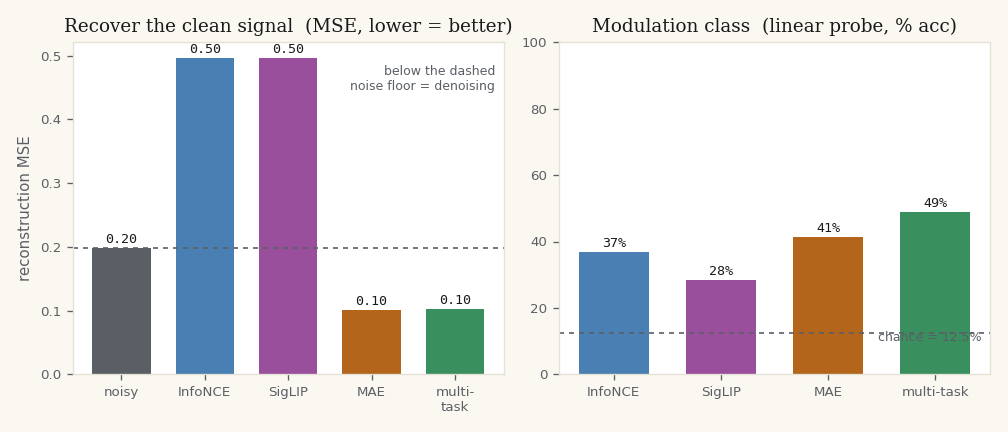
\includegraphics[width=\linewidth]{scores.png}
\caption{Left: recovering the clean signal. Both contrastive losses stay at $0.50$,
above the noise floor (dashed); reconstruction and multi-task denoise to $0.10$.
Right: linear-probe modulation class, where the multi-task model leads.}
\label{fig:scores}
\end{figure}

\begin{figure}[t]
\centering
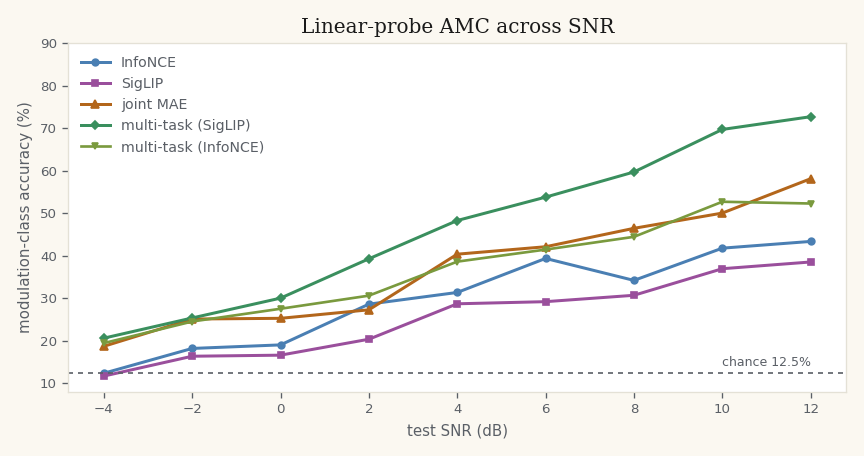
\includegraphics[width=\linewidth]{amc_snr.png}
\caption{Linear-probe AMC accuracy versus SNR. The SigLIP-head multi-task model leads
across the range, reconstruction and the InfoNCE-head multi-task model follow, and the
standalone contrastive encoders trail.}
\label{fig:amc}
\end{figure}

\begin{figure}[t]
\centering
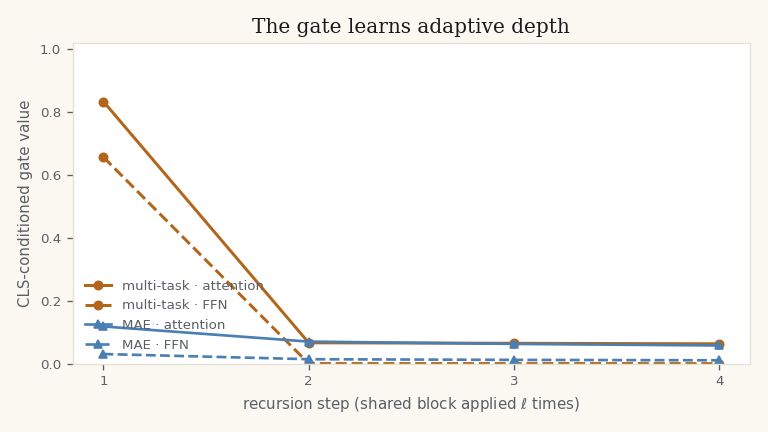
\includegraphics[width=\linewidth]{gates.png}
\caption{Mean CLS-conditioned gate value at each recursion step. Under the ponder
cost the gates collapse: the multi-task model keeps step~1 open and closes
steps~2--4, so the encoder learns it needs about one effective recursive
application.}
\label{fig:gates}
\end{figure}

\begin{figure}[t]
\centering
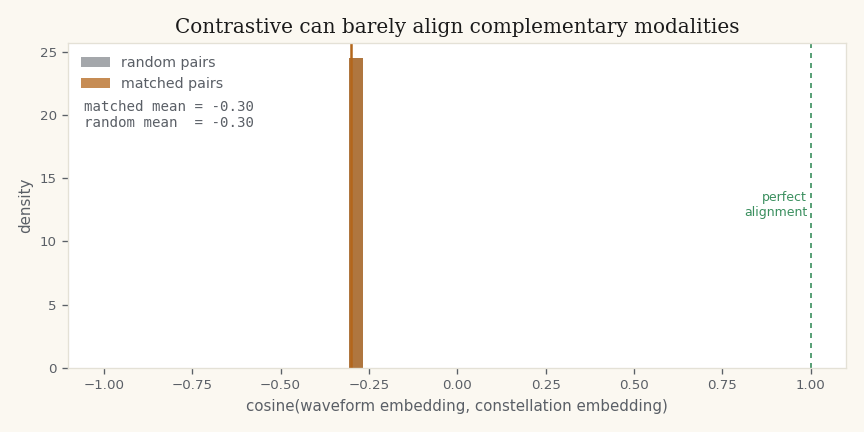
\includegraphics[width=\linewidth]{gap.png}
\caption{Contrastive alignment quality. Matched modality pairs reach a cosine far
from $1$, barely above random pairs: complementary modalities give alignment
little to grip.}
\label{fig:gap}
\end{figure}

\begin{figure}[t]
\centering
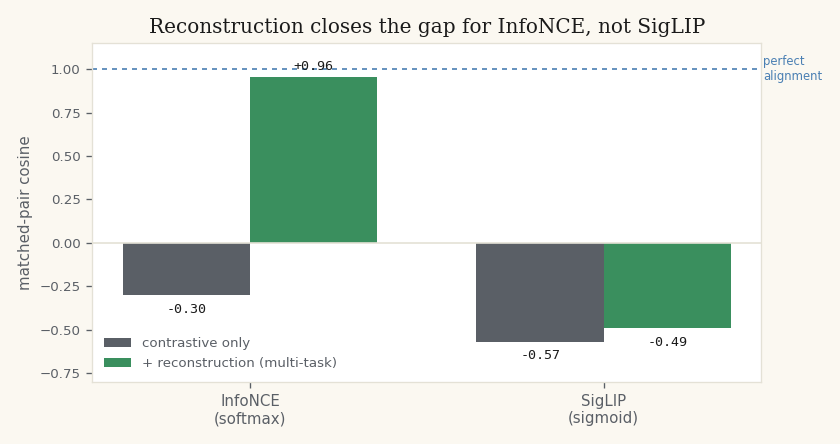
\includegraphics[width=\linewidth]{align.png}
\caption{Does reconstruction close the modality gap? Matched-pair cosine for each
contrastive head, standalone versus as a multi-task auxiliary to reconstruction.
The InfoNCE head closes the gap (to $+0.96$); the SigLIP head does not --- yet the
SigLIP head is the better classifier (Table~\ref{tab:recover}), so closing the gap
does not help.}
\label{fig:align}
\end{figure}

\begin{figure}[t]
\centering
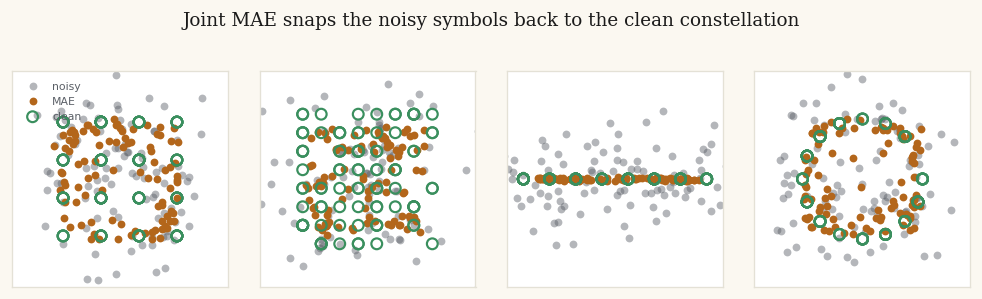
\includegraphics[width=\linewidth]{reconstruct.png}
\caption{The recursive MAE snaps noisy symbols (gray) back toward the clean
constellation (green); reconstruction in orange.}
\label{fig:reconstruct}
\end{figure}

\begin{thebibliography}{00}
\bibitem{oshea2018} T.~J. O'Shea, T.~Roy, and T.~C. Clancy, ``Over-the-air deep
learning based radio signal classification,'' \emph{IEEE J. Sel. Topics Signal
Process.}, 2018.
\bibitem{oshea2016} T.~J. O'Shea and N.~West, ``Radio machine learning dataset
generation with GNU Radio,'' \emph{Proc. GNU Radio Conf.}, 2016.
\bibitem{gardner} W.~A. Gardner, ``Exploitation of spectral redundancy in
cyclostationary signals,'' \emph{IEEE Signal Process. Mag.}, 1991.
\bibitem{dobre} O.~A. Dobre, A.~Abdi, Y.~Bar-Ness, and W.~Su, ``Survey of automatic
modulation classification techniques: Classical approaches and new trends,''
\emph{IET Commun.}, 2007.
\bibitem{finn} Y.~Umuroglu \emph{et al.}, ``FINN: A framework for fast, scalable
binarized neural network inference,'' \emph{FPGA}, 2017.
\bibitem{selfcontrastamc} D.~Liu, P.~Wang, T.~Wang, and T.~Abdelzaher,
``Self-contrastive learning based semi-supervised radio modulation classification,''
\emph{arXiv:2203.15932}, 2022.
\bibitem{kong} W.~Kong, X.~Jiao, Y.~Xu, B.~Zhang, and Q.~Yang, ``A transformer-based
contrastive semi-supervised learning framework for automatic modulation
recognition,'' \emph{IEEE Trans. Cogn. Commun. Netw.}, 2023.
\bibitem{denomae} A.~Faysal, T.~Bouhsine, M.~Rostami \emph{et al.}, ``DenoMAE: A
multimodal autoencoder for denoising modulation signals,'' \emph{arXiv:2501.11538},
2025.
\bibitem{denomae2} A.~Faysal, M.~Rostami, T.~Bouhsine \emph{et al.}, ``DenoMAE2.0:
Improving denoising masked autoencoders by classifying local patches for automatic
modulation classification,'' \emph{IEEE Trans. Commun.}, 2025.
\bibitem{mae} K.~He, X.~Chen, S.~Xie \emph{et al.}, ``Masked autoencoders are
scalable vision learners,'' \emph{CVPR}, 2022.
\bibitem{multimae} R.~Bachmann, D.~Mizrahi, A.~Atanov, and A.~Zamir, ``MultiMAE:
Multi-modal multi-task masked autoencoders,'' \emph{ECCV}, 2022.
\bibitem{ut} M.~Dehghani, S.~Gouws, O.~Vinyals, J.~Uszkoreit, and \L.~Kaiser,
``Universal transformers,'' \emph{ICLR}, 2019.
\bibitem{albert} Z.~Lan, M.~Chen, S.~Goodman \emph{et al.}, ``ALBERT: A lite BERT
for self-supervised learning of language representations,'' \emph{ICLR}, 2020.
\bibitem{highway} R.~K. Srivastava, K.~Greff, and J.~Schmidhuber, ``Highway
networks,'' \emph{arXiv:1505.00387}, 2015.
\bibitem{rezero} T.~Bachlechner \emph{et al.}, ``ReZero is all you need: Fast
convergence at large depth,'' \emph{UAI}, 2021.
\bibitem{layerscale} H.~Touvron \emph{et al.}, ``Going deeper with image
transformers (CaiT),'' \emph{ICCV}, 2021.
\bibitem{act} A.~Graves, ``Adaptive computation time for recurrent neural
networks,'' \emph{arXiv:1603.08983}, 2016.
\bibitem{pondernet} A.~Banino, J.~Balaguer, and C.~Blundell, ``PonderNet:
Learning to ponder,'' \emph{ICML Workshop}, 2021.
\bibitem{mod} D.~Raposo, S.~Ritter, B.~Richards \emph{et al.}, ``Mixture-of-Depths:
Dynamically allocating compute in transformer-based language models,''
\emph{arXiv:2404.02258}, 2024.
\bibitem{looped} A.~Giannou, S.~Rajput, J.~Sohn \emph{et al.}, ``Looped
transformers as programmable computers,'' \emph{ICML}, 2023.
\bibitem{relaxedrec} S.~Bae, A.~Fisch, H.~Harutyunyan \emph{et al.}, ``Relaxed
recursive transformers: Effective parameter sharing with layer-wise LoRA,''
\emph{arXiv:2410.20672}, 2024.
\bibitem{mor} S.~Bae, Y.~Kim, R.~Bayat \emph{et al.}, ``Mixture-of-Recursions:
Learning dynamic recursive depths for adaptive token-level computation,''
\emph{arXiv:2507.10524}, 2025.
\bibitem{cotformer} A.~Mohtashami, M.~Pagliardini, and M.~Jaggi, ``CoTFormer: A
chain-of-thought driven architecture with budget-adaptive computation cost at
inference,'' \emph{arXiv:2310.10845}, 2023.
\bibitem{sut} S.~Tan, Y.~Shen, Z.~Chen, A.~Courville, and C.~Gan, ``Sparse universal
transformer,'' \emph{EMNLP}, 2023.
\bibitem{depthadaptive} M.~Elbayad, J.~Gu, E.~Grave, and M.~Auli, ``Depth-adaptive
transformer,'' \emph{ICLR}, 2020.
\bibitem{sact} M.~Figurnov \emph{et al.}, ``Spatially adaptive computation time for
residual networks,'' \emph{CVPR}, 2017.
\bibitem{gtrxl} E.~Parisotto \emph{et al.}, ``Stabilizing transformers for
reinforcement learning,'' \emph{ICML}, 2020.
\bibitem{deebert} J.~Xin, R.~Tang, J.~Lee, Y.~Yu, and J.~Lin, ``DeeBERT: Dynamic
early exiting for accelerating BERT inference,'' \emph{ACL}, 2020.
\bibitem{pabee} W.~Zhou \emph{et al.}, ``BERT loses patience: Fast and robust
inference with early exit,'' \emph{NeurIPS}, 2020.
\bibitem{cavmae} Y.~Gong \emph{et al.}, ``Contrastive audio-visual masked
autoencoder,'' \emph{ICLR}, 2023.
\bibitem{m3ae} X.~Geng \emph{et al.}, ``Multimodal masked autoencoders learn
transferable representations,'' \emph{arXiv:2205.14204}, 2022.
\bibitem{zorro} A.~Recasens \emph{et al.}, ``Zorro: The masked multimodal
transformer,'' \emph{arXiv:2301.09595}, 2023.
\bibitem{cavmaesync} E.~Araujo \emph{et al.}, ``CAV-MAE Sync: Improving contrastive
audio-visual masked autoencoders via fine-grained alignment,'' \emph{CVPR}, 2025.
\bibitem{clip} A.~Radford \emph{et al.}, ``Learning transferable visual models
from natural language supervision,'' \emph{ICML}, 2021.
\bibitem{siglip} X.~Zhai, B.~Mustafa, A.~Kolesnikov, and L.~Beyer, ``Sigmoid loss
for language image pre-training,'' \emph{ICCV}, 2023.
\bibitem{modgap} W.~Liang \emph{et al.}, ``Mind the gap: Understanding the modality
gap in multi-modal contrastive representation learning,'' \emph{NeurIPS}, 2022.
\bibitem{schrodi} S.~Schrodi, D.~T. Hoffmann, M.~Argus, V.~Fischer, and T.~Brox,
``Two effects, one trigger: On the modality gap, object bias, and information
imbalance in contrastive vision-language models,'' \emph{ICLR}, 2025.
\bibitem{fahim} A.~Fahim, A.~Murphy, and A.~Fyshe, ``It's not a modality gap:
Characterizing and addressing the contrastive gap,'' \emph{arXiv:2405.18570}, 2024.
\bibitem{modcl} C.~Wang, S.~Wang, L.~Han \emph{et al.}, ``Modulation
consistency-based contrastive learning for self-supervised automatic modulation
classification,'' \emph{arXiv:2605.11875}, 2026.
\bibitem{pid} P.~P. Liang \emph{et al.}, ``Quantifying \& modeling multimodal
interactions: An information decomposition framework,'' \emph{NeurIPS}, 2023.
\bibitem{bertschinger} N.~Bertschinger, J.~Rauh, E.~Olbrich, J.~Jost, and N.~Ay,
``Quantifying unique information,'' \emph{Entropy}, 2014.
\bibitem{tschannen} M.~Tschannen, J.~Djolonga, P.~K. Rubenstein, S.~Gelly, and
M.~Lucic, ``On mutual information maximization for representation learning,''
\emph{ICLR}, 2020.
\end{thebibliography}

\appendix
\section{Modalities and Benchmark Construction}
\label{app:modalities}
We instantiate the two modalities, in the spirit of the DenoMAE
family~\cite{denomae,denomae2}, as explicit lossy projections of the clean signal. Let $Z$ be a length-$M$ sequence
of symbols drawn from one of $K$ modulation schemes. The receiver observes
\begin{align}
X_{\text{wav}} &= Z + \eta, &
X_{\text{con}} &= \mathrm{Hist}_{G\times G}(Z+\eta),
\end{align}
where $\eta$ is additive white Gaussian noise at a given SNR. The waveform
$X_{\text{wav}}$ keeps symbol order but is noisy; the constellation $X_{\text{con}}$,
a 2D I/Q histogram, keeps clean cluster geometry but discards order. Recovering $Z$
therefore needs order from the waveform and geometry from the constellation, so the
two views are complementary rather than redundant; this is the structural fact the
align-versus-reconstruct analysis rests on.

The benchmark draws $K{=}8$ schemes (BPSK, QPSK, 8PSK, 16QAM, 64QAM, 4PAM, 8PAM,
16PSK) with $M{=}96$ symbols per example and a $G{=}24$ constellation histogram.
Representations are pretrained on signals at SNR sampled uniformly from
$[-2,10]$\,dB and evaluated from $-4$ to $12$\,dB, matching the DenoMAE-style
across-SNR AMC protocol of Sec.~\ref{sec:setup}.

\section{Contrastive Objectives}
\label{app:contrastive}
Our contrastive variants are the standard CLIP and SigLIP losses, used unmodified
and restated here for completeness. Given L2-normalized per-modality \texttt{[CLS]}
embeddings $\bm{z}^{\text{wav}}, \bm{z}^{\text{con}}$, the softmax InfoNCE loss of
CLIP~\cite{clip} is
\begin{equation}
\mathcal{L}_{\text{InfoNCE}} = -\frac{1}{N}\sum_i
\log\frac{\exp(\bm{z}^{\text{wav}}_i\!\cdot \bm{z}^{\text{con}}_i/\tau)}
{\sum_j \exp(\bm{z}^{\text{wav}}_i\!\cdot \bm{z}^{\text{con}}_j/\tau)},
\end{equation}
with temperature $\tau$. The SigLIP~\cite{siglip} pairwise-sigmoid alternative is
\begin{equation}
\mathcal{L}_{\text{SigLIP}} = \sum_{i,j}\mathrm{softplus}\!\big(-y_{ij}\,(t\,
\bm{z}^{\text{wav}}_i\!\cdot\bm{z}^{\text{con}}_j + b)\big),
\end{equation}
with $y_{ii}=1$, $y_{i\neq j}=-1$ and learned scale and bias $t,b$. In the
multi-task objective $\mathcal{L}_{\text{SigLIP}}$ is the contrastive term scaled by
$\lambda_{\text{c}}$.

\end{document}
